\section{Polynomdivision}\index{Polynomdivision}
Die Polynomdivision wird eingesetzt um entweder den Grad eines Polynoms zu verringern oder die Bruchform einer gebrochenrationalen Funktion in die Summenform umzuwandeln.
\subsection{Polynomdivision bei Polynomen}\index{Polynomdivision!Polynome}\label{polynomdivision}

    Bei einem Polynom wird die Polynomdivision angewendet um den Grad des Polynoms zu verringern und die Faktorisierte Darstellung des Polynoms zu erzeugen. Als Beispiel wird hier die Funktion $f(x) = x^3-6x^2-x+6$ verwendet. Hierbei ist es Ziel, dass man das Polynom als Produkt der Nullstellen darstellen kann.\\
    Es gilt folgender Zusammenhang: $$f(x) = x^3-6x^2-x+6 =  \polyfactorize{x^3-6x^2-x+6}.$$ Aus dieser Darstellung folgt, dass die Funktion $f$ die Nullstellen $x_1 = -1, x_2 = 1$ und $x_3= 6$ hat. Um die Polynomdivision durchführen zu können, muss man als erstes eine Nullstelle kennen und dann das Polynom durch diese Nullstelle teilen. Nach der Division erhält man jeweils eine neues Polynom geringeren Grades. Dieses Polynom muss dann wieder mit der Polynomdivision vom Grad reduziert werden.
    \begin{bsp}{Die Polynomdivision bei Polynomen}{} 
Man rät die Nullstelle $x=1$ und führt jetzt die Polynomdivision durch:\\
 \polylongdiv{x^3- 6x^2 - x +6}{x-1}\\
 Das neue Polynom kann jetzt mit der Mitternachtsformel weiter bearbeitet werden oder erneut durch eine Polynomdivision bearbeitet werden. \\
  \polylongdiv{x^2-5x^1 -6}{x+1}\\
  oder
  $$ x_{1,2} = \dfrac{5\pm \sqrt{(-5)^2 - 4\cdot 1 \cdot (-6)}}{2\cdot 1} = \dfrac{5 \pm \sqrt{49} }{2} = \dfrac{5\pm 7}{2}$$
 $$ x_1 = -1$$
 $$ x_2= 6$$
\begin{center}
    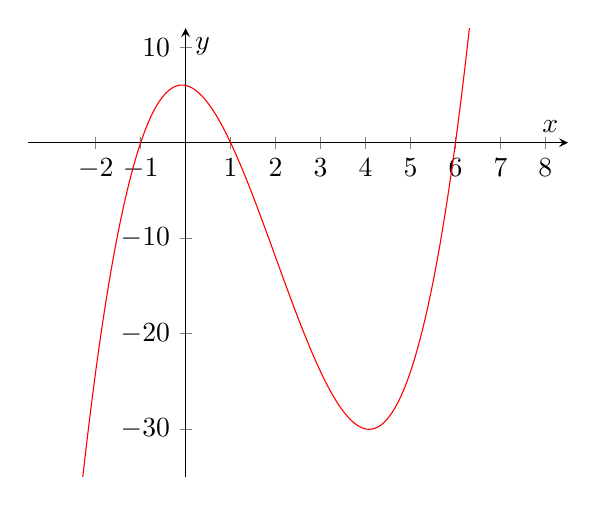
\begin{tikzpicture}
        \begin{axis}[xmin= -3.5, xmax = 8.5, ymin= -35, ymax= 12,
        axis lines = middle, 
        xtick={-2, -1, 0, ..., 8},
        xlabel = $x$,
        ylabel=$y$]
            \addplot[color= red, samples = 300, domain= -2.5:6.5]{x^3-6*x^2-x+6};
        \end{axis}
    \end{tikzpicture}     
\end{center}
\end{bsp}
\begin{b8d}{Rest der Polynomdivision}{rest}
  Bei der Polynomdivision zur Bestimmung der Nullstellen eines Polynoms treten \textcolor{red}{keine Restterme} auf.   
\end{b8d}
\subsection{Polynomdivision bei gebrochenrationalen Funktionen}\index{Polynomdivision!gebrochenrationale Funktionen}\label{polynomdivisionBruch}
Die zweite Anwendung der Polynomdivision besteht in der Umwandlung der Bruchform in die Summenform der ganzrationalen Funktionen. Hierbei wird die Polynomdivision durchgeführt indem man den Zähler der Funktion durch seinen Nenner dividiert.
\begin{bsp}{Polynomdivision ganzrationaler Funktionen}{}
Gegeben ist die Funktion $$f(x)=\dfrac{x^2+x-2}{2x-4}$$ mit $\mathds{D}_f=\mathds{R}\setminus \left\{ 2 \right\}$. Durch die Polynomdivision soll die Bruchform in die Summenform überführt werden.\\
\polylongdiv{x^2+x-2}{2x-4}\\
Damit lautet die Summenform wie folgt:
$$f(x)=\dfrac{x^2+x-2}{2x-4} = \dfrac{1}{2} x +\dfrac{3}{2} +\dfrac{4}{2x-4} $$
\end{bsp}
\subsection{Symmetrie} \index{Symmetrie}
Die Untersuchung der Symmetrie erfolgt für Funktionen immer nach dem selben Muster. Es wird im allgemeinen Untersucht, ob entweder \begin{equation}\label{f(x)}
    f(-x) = f(x)
\end{equation} oder 
\begin{equation} \label{-f(x)}
f(-x) = -f(x) 
\end{equation} gilt. Für die Gleichung \ref{f(x)} ist der Graph der Funktion $f$ achsensymmetrisch zur y-Achse. Für die Gleichung \ref{-f(x)} ist der Graph der Funktion $f$ punktsymmetrisch zum Ursprung. Gilt keine der beiden Gleichungen kann keine Aussage zur Symmetrie zur y-Achse bzw. zum Ursprung getroffen werden. 
\begin{center}
    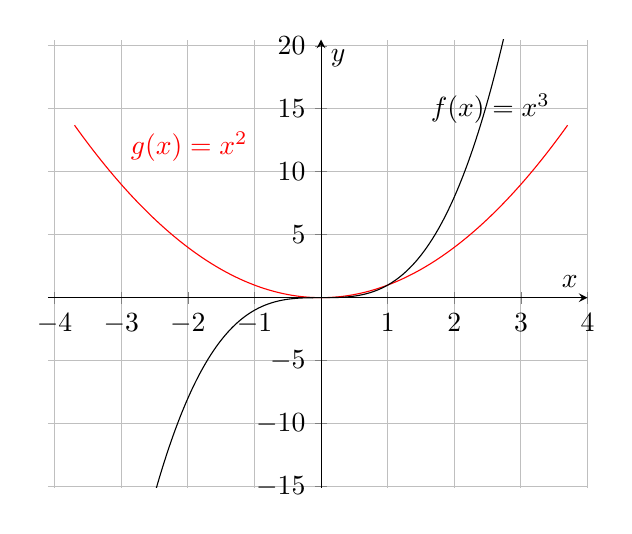
\begin{tikzpicture}
        \begin{axis}[xmin= -4.1, xmax = 4, ymin= -15.1, ymax= 20.5,
        axis lines = middle, 
        ymajorgrids=true,
        xmajorgrids=true,
        xtick={-4, -3,  ..., 2, 3, 4},
        ytick={-15, -10, -5, ..., 20},
        xlabel = $x$,
        ylabel=$y$]
            \addplot[color = red, samples = 300, domain= -3.7:3.7]{x^2};
         \draw (1.5,15)   node [right] {$f(x) = x^3$};  
            \addplot[color= black, samples = 300, domain= -3.7:3.7]{x^3};
            \draw (-3,12)   node [right] {\textcolor{red}{$g(x) = x^2$}}; 
            
        \end{axis}
    \end{tikzpicture}  
\end{center}
\section{Übersicht von Ableitungsregeln} \index{Ableitung! Übersicht}